\section*{Введение}
Целью разрабатываемого программного продукта является обеспечение простого и удобного ведение собственной информационной базы, включающей в себя систему ведения заметок и категорированных закладок.

Каждый день человек сталкивается со множество информации, которую необходимо запомнить и использовать в дальнейшем, но вследствие человеческого фактора данная информация может быть забыта или утеряна. Для того, чтобы выносить ключевые моменты из обработанного материала, необходима система, которая бы позволяла просто и удобно реализовывать эту задачу. В большинстве случаев разработанный продукт будет актуален студентам и работникам различных научных направлений, так как именно в перечисленных сферах чаще всего возникает потребность в постоянном поиске и обработке информации.

Для разработки системы необходимо выполнить следующие задачи:
\begin{itemize}
	\item анализ предметной области;
	\item формирование функциональных требований к системе;
	\item серверное веб-приложение;
        \item клиентское веб-приложение;
        \item плагин для браузера;
        \item тестирование разработанной системы.
\end{itemize}

\addcontentsline{toc}{section}{Постановка задачи}

\newpage
\section{Общее описание}
Назначением разработанного проекта является помощь человеку разгрузить свою «оперативную память», предоставляя возможность вести список заметок и закладок, к которым пользователь может обратиться в любой момент с любого устройства.

Большинство приложений с функционалом создания заметок и закладок, требуют от пользователя знаний и умений работы в конкретном сервисе. Однако это отнимает много времени, а необходимость в записи информации может возникнуть в любой момент. Начинающий пользователь может запутаться или записать в заметках телефона без желания опробовать интерфейс. Можно сделать вывод о том, что крайне не хватает приложения с удобным интерфейсом и направленным функционалом. Поэтому наша команда с удовольствием взялась за разработку такого решения и поставила следующую цель: обеспечить простое и удобное ведение собственной базы данных, с возможностью ведения заметок и добавления закладок.

\section{Интерфейсы системы}
Разработанный сервис позволяет создать закладку используя такие данные, как URL сайта и его название. Закладку можно удалить, изменить и скопировать. С помощью нажатия на кнопку “Перейти” вы сможете перейти на сайт из закладки. Также реализована возможность сортировки закладок по какому-либо признаку и поиска, что позволяет легко работать с большим объемом информации.

\begin{figure}[H]
	\begin{center}
		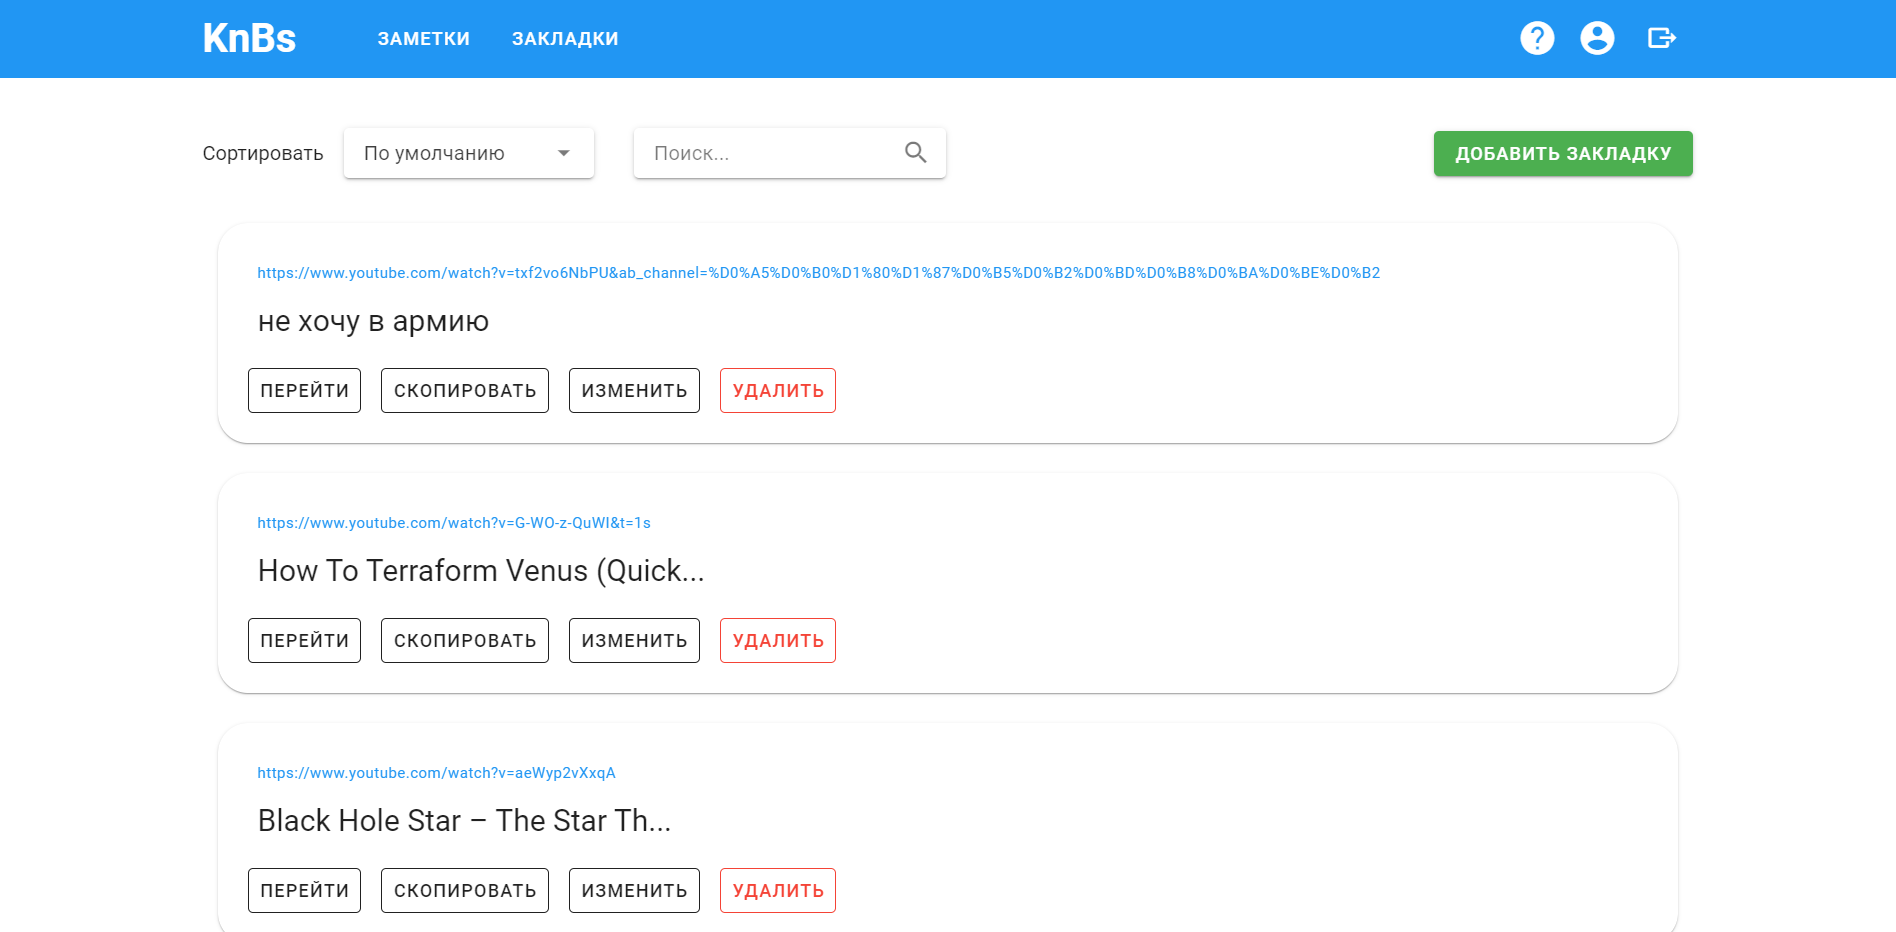
\includegraphics[scale=0.25]{bookmarks}
		\caption{Страница закладок}
		\label{pic:bookmarks} % название для ссылок внутри кода
	\end{center}
\end{figure}

На странице «Заметки» отображается весь список добавленных заметок. Заметки можно изменять, а также удалять не нужные, используя необходимые кнопки. Для добавления необходимо ввести название и нужную вам информацию, после чего нажать на кнопку «Добавить», и заметка появится в общем списке. Для заметок был расширен функционал сортировки, в отличии от закладок. Заметки можно сортировать по умолчанию, по дате создания, по дате редактирования, по названию. Также, как и в создании закладок, реализована возможность поиска.

\begin{figure}[H]
	\begin{center}
		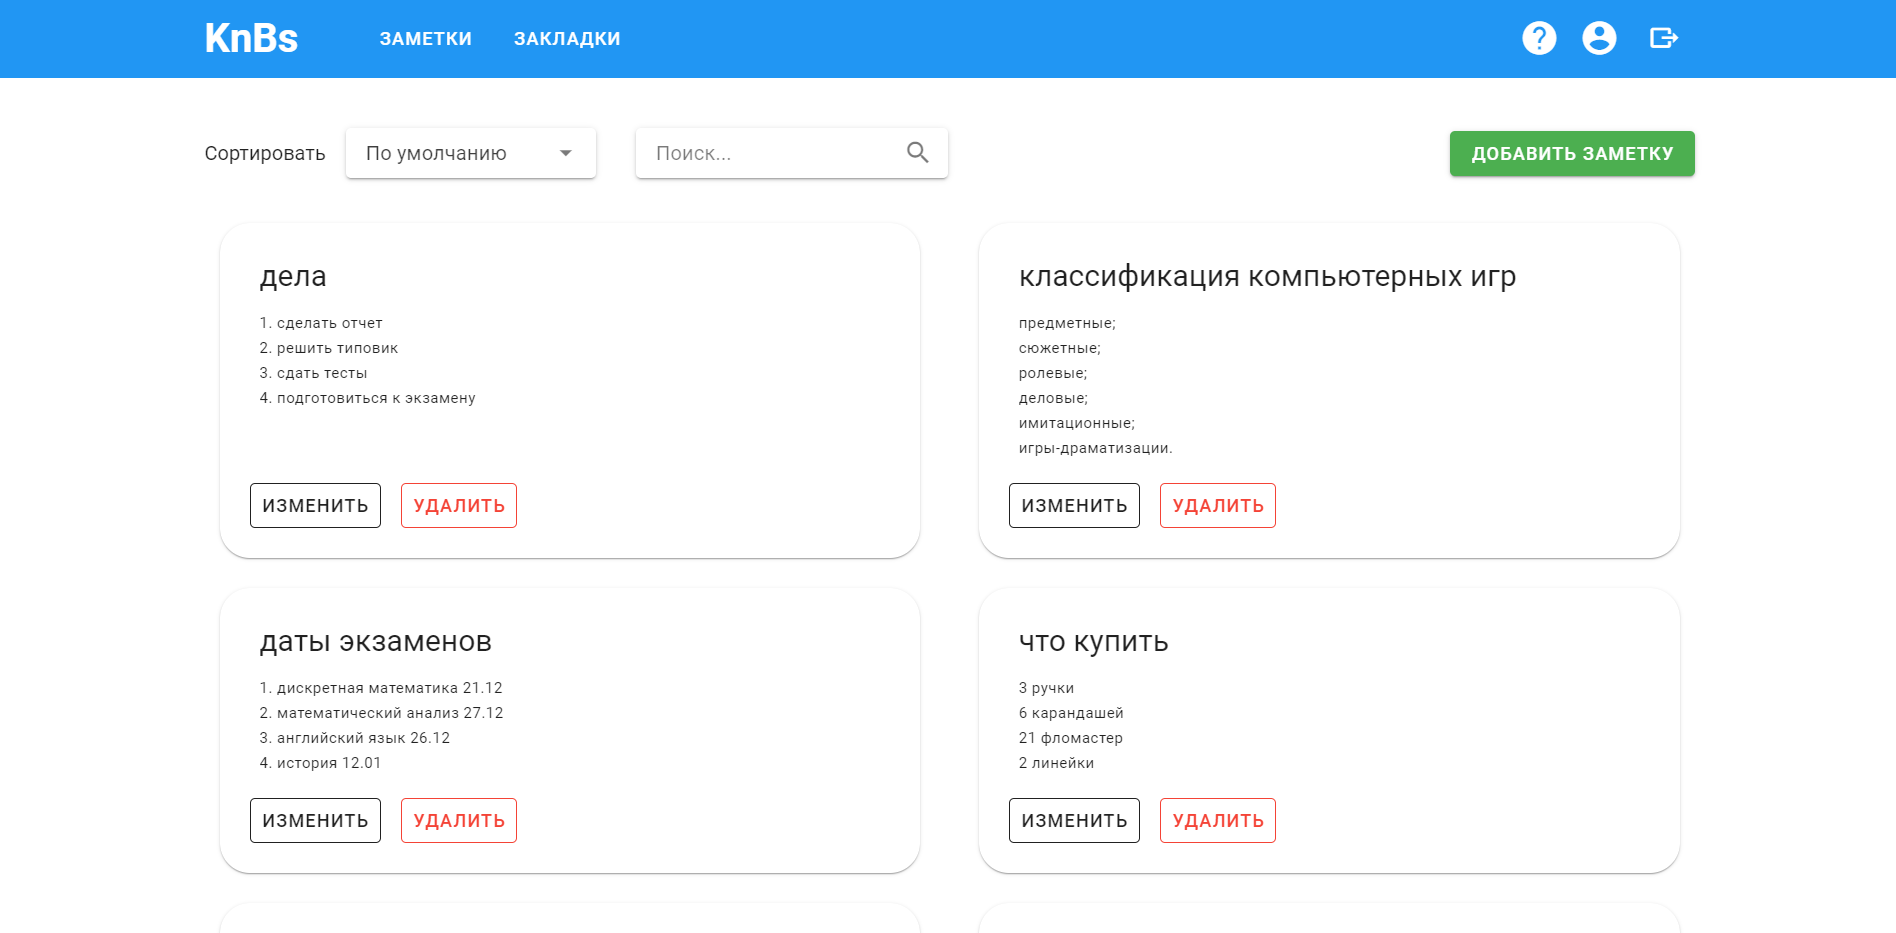
\includegraphics[scale=0.25]{notes}
		\caption{Схема неструктурированной сети}
		\label{pic:notes} % название для ссылок внутри кода
	\end{center}
\end{figure}

Наше приложение может быть запущено как на удаленном сервере, так и локально на компьютере пользователя, что дает возможность работать с ним даже без доступа в интернет. Для подключения к серверу и сохранения закладок необходимо ввести его адрес в соответствующее поле в окне расширения. Также пользователь должен ввести свой ключ доступа к приложению, с помощью которого происходит авторизация для того, чтобы получить доступ к созданию закладок.

\section{Выбор архитектуры системы}

Веб-приложение – клиент-серверное приложение, в котором клиент взаимодействует с веб-сервером при помощи браузера. Логика веб-приложения распределена между сервером и клиентом, хранение данных осуществляется, преимущественно, на сервере, обмен информацией происходит по сети. Одно из преимуществ такого подхода это независимость клиентов от конкретной операционной системы.
Рекомендовано ознакомиться с сайтом ~\cite{PortalTpu}

\section{Обоснование выбора технологий и программных средств}

Для разработки веб-сервиса был выбран язык программирования JavaScript – является одним из самых популярных языков программирования.

Именно в области Frontend задействовано огромное число наработок, основанных на Javascript. Наиболее активно используется примерно 25-30 библиотек и фреймворков. Эти готовые шаблоны и решения для стандартных задач существенно экономят время. Они упрощают процесс web-разработки, ускоряют его, снижая стоимость проектов.

Рекомендовано ознакомиться с книгой ~\cite{JsBook} для более подробного изучения JavaScript.

В таблице ~\ref{tab:tab1} приведен сравнительный анализ популярных фреймворков для разработки на языке JavaScript.

\begin{table}[H]
    \caption{Сравнительный анализ популярных фреймворков}
    \begin{center}
        \begin{tabular}{|c|c|c|c|}
            \hline
                \begin{tabular}[c]{@{}l@{}}Критерий\end{tabular} &
                \begin{tabular}[c]{@{}l@{}}Vue.js\end{tabular} &
                \begin{tabular}[c]{@{}l@{}}React.js\end{tabular} &
                \begin{tabular}[c]{@{}l@{}}Angular\end{tabular} \\
            \hline
                Рендеринг &
                \begin{tabular}[c]{@{}l@{}}создается копия \\ DOM\end{tabular} &
                \begin{tabular}[c]{@{}l@{}}создается копия \\ DOM\end{tabular} &
                \begin{tabular}[c]{@{}l@{}}рендеринг HTML-страниц \\ на стороне сервера\end{tabular} \\
            \hline
                \begin{tabular}[c]{@{}l@{}}Архитектура \\ компонентов \end{tabular} &
                \begin{tabular}[c]{@{}l@{}}Высокоуровневый \\ API обеспечивает \\ совместимость для \\ всех библиотек\end{tabular} &
                \begin{tabular}[c]{@{}l@{}}Необходим поиск \\ и внедрение \\ дополнительных \\ библиотек\end{tabular} &
                \begin{tabular}[c]{@{}l@{}}Необходим поиск и \\ внедрение дополнительных \\ библиотек\end{tabular} \\
            \hline
                \begin{tabular}[c]{@{}l@{}}Двустороннее \\ связывание \end{tabular} &
                есть &
                нет &
                есть \\ 
            \hline
                \begin{tabular}[c]{@{}l@{}}Декомпозиция \\ объектов\end{tabular} &
                есть &
                есть &
                есть \\ 
            \hline
                Представление &
                \begin{tabular}[c]{@{}l@{}}HTML-шаблоны \\ и JSX\end{tabular} &
                JSX &
                \begin{tabular}[c]{@{}l@{}}HTML-шаблоны и JSX\end{tabular} \\ 
            \hline
        \end{tabular}
        \label{tab:tab1}
    \end{center}
\end{table}

Vue.js – прогрессивный фреймворк с подробно прописанной документацией и множеством примеров. Он позволяет создавать переиспользуемые компоненты за счет архитектурных особенностей фреймворка. Для увеличения производительности Vue.js использует виртуальную копию DOM, а для сохранения целостности данных этот фреймворк поддерживает двустороннее связывание, поэтому для написания front-end проекта был выбран именно Vue.js.

В качестве серверной разработки была выбрана платформа Firebase для разработки мобильных и веб-приложений. Firebase — это облачная база данных, которая позволяет пользователям хранить и получать сохраненную информацию, а также имеет удобные средства и методы взаимодействия с ней.

Firebase хранит текстовые данные в JSON формате и предоставляет удобные методы для чтения, обновления и извлечения данных. Также, Firebase может помочь с регистрацией и авторизацией пользователей, хранением сессий (авторизованные пользователи), медиафайлов к которым с легкостью предоставляет доступ благодаря Cloud Storage.

Также считаю нужным поделится разработанной мною формулой для зароботка денег ~\ref{eq:eq1}.

\begin{equation}\label{eq:eq1}\tag{1}
\end{equation}
$$
M(x) = J + \sum \limits_{n=5}^{\infty} I_n + \sin \left( \frac{2 \pi x}{\nu} - W_n \right) \eqno (1)
$$

Воспользовавшись ее вы останетесь с деньгами после новогодних празников. С наступающим новым годом!

\newpage
\section{Листинг}
\begin{code}
	\inputminted[breaklines=true, xleftmargin=1em, linenos, frame=single, framesep=10pt, fontsize=\footnotesize]{haskell}{listings/NotesView.vue}
	\caption{Листинг страницы закладок}
\end{code}

\newpage
\section*{Заключение}
В результате выполнения курсового проекта была полностью выполнена основная цель разрабатываемого продукта, удалось создать веб-приложение для предоставления пользователям возможности управления собственной информационной базы «Knowledge Base».

Моей задачей в проекте являлось проектирование архитектуры клиентской части веб-приложение, а также контроль над остальными участниками команды frontend-разработчиков. Мною была размечена структура проекта, настроено окружение и подключены необходимые зависимости. Также сверстаны страницы авторизации и регистрации пользователей.

В дальнейший план развития проекта входит реализация следующих задач:

\begin{itemize}
	\item возможность добавления нового функционала для выстраивания взаимосвязей между заметками и закладками;
	\item мобильное приложение для Android и IOS.
\end{itemize}

\addcontentsline{toc}{section}{Заключение}